% Copyright 2020 by Junwei Wang <i.junwei.wang@gmail.com>
%
% This file may be distributed and/or modified under the
% conditions of the LaTeX Project Public License, either version 1.3c
% of this license or (at your option) any later version.
% The latest version of this license is in
%   http://www.latex-project.org/lppl.txt

% \documentclass[aspectratio=169,compress]{beamer}
\documentclass[aspectratio=169,compress]{beamer}

\usepackage[english]{babel}
\usepackage{metalogo}
\usepackage{listings}
\usepackage{fontspec}
\usepackage{tikz}

% \usetheme{Nord}
\usetheme[style=light]{Nord}


%\usepackage[spanish, es-tabla]{babel}
\usepackage[utf8]{inputenc}
\usepackage{hyperref}




\setmainfont{Yanone Kaffeesatz}
%\setsansfont{Andika New Basic}
\setmonofont{DejaVu Sans Mono}

\setbeamerfont{frametitle}{parent=structure,size=\Large}

\AtBeginSection[]
{
  \begin{frame}[c,noframenumbering,plain]
    \tableofcontents[sectionstyle=show/hide,subsectionstyle=show/show/hide]
  \end{frame}
}

\AtBeginSubsection[]
{
  \begin{frame}[c,noframenumbering,plain]
    \tableofcontents[sectionstyle=show/hide,subsectionstyle=show/shaded/hide]
  \end{frame}
}

\title{Arquitecturas y Organización de Computadoras I}
\subtitle{4: Microarquitectura/Organización: Segmentación (paralelismo a nivel de instrucciones)}
\author{Rafael Ignacio Zurita}
\institute{Depto. Ingeniería de Computadoras}
\date{\today}

\begin{document} 
\begin{frame}[plain,noframenumbering]
\bigskip
  \maketitle
\end{frame}





\begin{footnotesize}

\section{Segmentación (Pipeling)}




\begin{frame}{Temario}{UNIDAD 5 - Introducción a las Arquitecturas Modernas}
\begin{itemize}
\item Camino de datos segmentado
\item Mejora de rendimiento
\item Nuevos elementos en la arquitectura
\item Problemas en la segmentación
\end{itemize}
\end{frame}




\begin{frame}
\frametitle{Temario}
        \begin{center}
        \textbf{Microarquitectura}
        \end{center}
\begin{tabular}{cl}

\begin{tabular}{c}
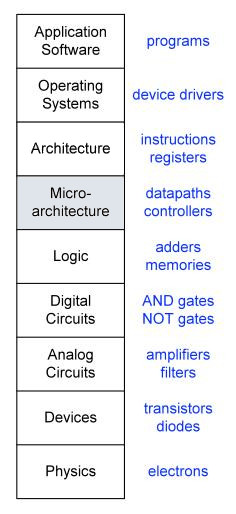
\includegraphics[height=6cm, width=4cm]{images/estructura-por-niveles.jpg} 

\end{tabular}
& \begin{tabular}{l}
\parbox{0.5\linewidth}{
        Como implementar una arquitectura en hardware (meta: costo, rendimiento, etc) \\ \\
        La microarquitectura es construída por circuitos lógicos y elementos de memoria \\ \\
        Todos los circuitos lógicos y elementos de memoria son implementados físicamente con transistores
}
\end{tabular} \\

\end{tabular}
\end{frame}





\begin{frame}
\frametitle{Implementación de la Microarquitectura}
\begin{center}\textbf{Diseño de la Microarquitectura (diseño del procesador)}\end{center}
\begin{enumerate}
\item Analizar el conjunto de instrucciones (ISA)
\begin{itemize}
\item Obtener los requerimientos del camino de datos
\end{itemize}
\item Seleccionar los \textit{componentes} y establecer la \textit{metodología} del reloj
\item Componer el \textit{camino de datos} para cumplir los requerimientos
\item Determinar las \textit{señales de control} para cada instrucción
\item Componer la \textit{lógica de control (unidad de control)} para generar las señales de control
\end{enumerate}
\end{frame}



\begin{frame}
\frametitle{Implementación de la Microarquitectura}
\begin{center}\textbf{Microarquitectura segmentada }\end{center}
\begin{itemize}
\item Uso de varias unidades al mismo
\item Compartir elementos entre diferentes instrucciones
\item \textbf{Paralelismo a nivel de instrucciones}
\end{itemize}
\end{frame}



\subsection{Ejemplo de segmentación y paralelismo en una lavandería}

\begin{frame}
\frametitle{Implementación de la Microarquitectura}
\begin{center}\textbf{Ejemplo de la lavandería}\end{center}
\begin{itemize}
\item Problema de trabajo
\begin{itemize}
\item Cuatro etapas de tareas
\item Tiempos balanceados (aprox. 30 min.)
\item Secuencia fija de pasos
\item Tiempo total para n trabajos = (n * 2hs.)
\end{itemize}
\end{itemize}
\begin{figure}
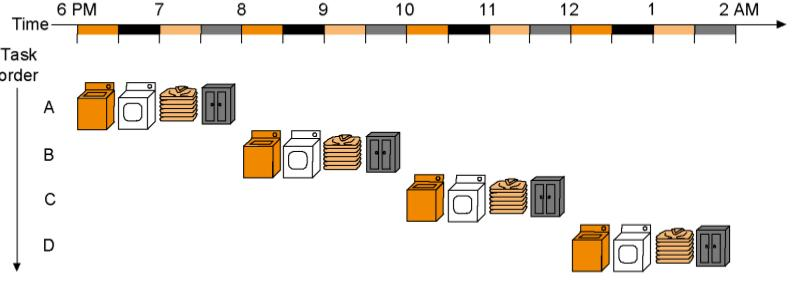
\includegraphics[scale=0.4]{images/lavanderia1.jpg} 
\end{figure}
\end{frame}




\begin{frame}
\frametitle{Implementación de la Microarquitectura}
\begin{center}\textbf{Ejemplo de la lavandería}\end{center}
\begin{itemize}
\item Optimizacion real
\begin{itemize}
\item Las unidades operan independientemente
\item Se pueden utilizar unidades al mismo tiempo
\item Tiempo promedio por lavado similar al anterior
\item Tiempo total para n cargas = aprox. (n * tiempo por etapa)
\end{itemize}
\end{itemize}
\begin{figure}
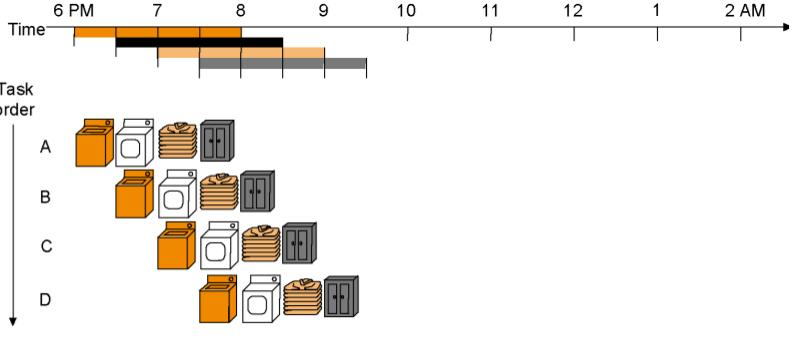
\includegraphics[scale=0.4]{images/lavanderia2.jpg} 
\end{figure}
\end{frame}


\subsection{Diseño mejorado - Registros buffers}


\begin{frame}
\frametitle{Implementación de la Microarquitectura}
\begin{center}\textbf{Precondiciones}\end{center}
\begin{itemize}
\item Diseño del conjunto de instrucciones
\begin{itemize}
\item Instrucciones de ancho fijo (idealmente)
\item Pocos formatos de instrucciones
\item Operandos en memoria sólo para instrucciones de carga y almacenamiento
\item Datos alineados
\end{itemize}
\end{itemize}
\begin{itemize}
\item Origen de los problemas
\begin{itemize}
\item Instrucciones con longitud variable
\item Datos no alineados
\end{itemize}
\end{itemize}

\end{frame}








\begin{frame}
\frametitle{Implementación de la Microarquitectura}
\begin{center}\textbf{Camino de datos de un ciclo}\end{center}
\begin{figure}
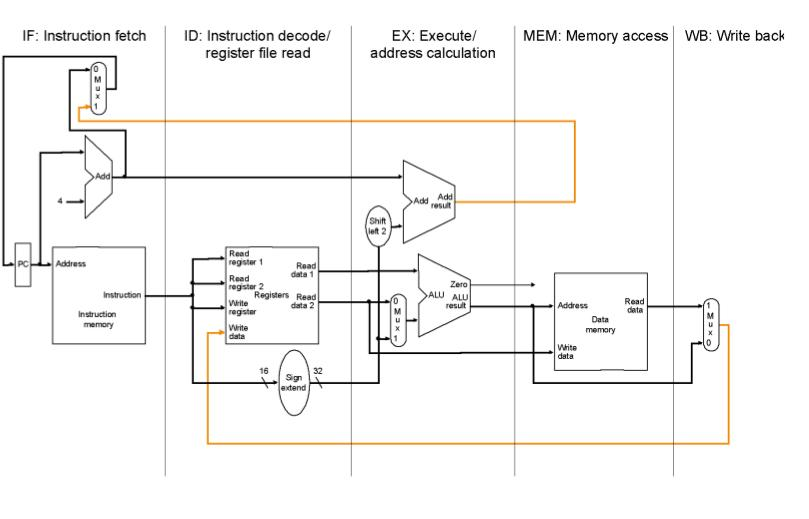
\includegraphics[scale=0.3]{images/single.jpg} 
\end{figure}

\end{frame}




\begin{frame}
\frametitle{Implementación de la Microarquitectura}
\begin{center}\textbf{Camino de datos segmentado}\end{center}
\begin{figure}
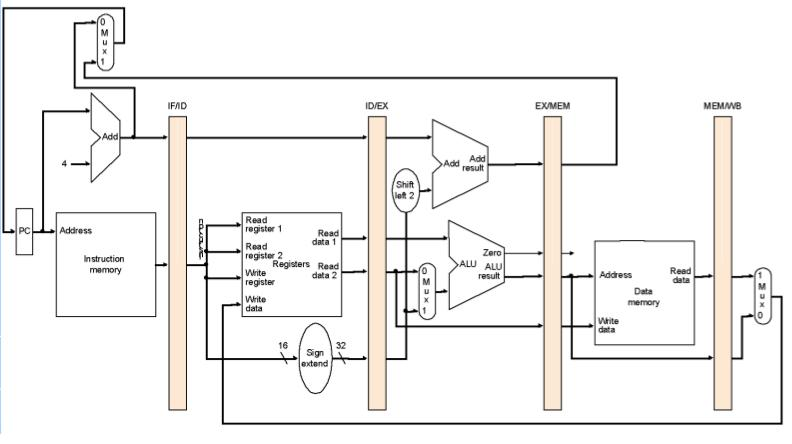
\includegraphics[scale=0.3]{images/pipelined.jpg} 
\end{figure}

\end{frame}



\begin{frame}{Camino de datos segmentado}{Etapas}
\begin{center}\textbf{Camino de datos segmentado}\end{center}
\begin{itemize}
\item Idea clave: aumentar la productividad (no la latencia)
\item Hardware mas complejo: registros de la microarquitectura
\item Posibilita un incremento de la frecuencia del reloj
\end{itemize}

\end{frame}



\subsection{Mejora del rendimiento}

\begin{frame}{Mejora del rendimiento con la segmentación}{Tiempo de ejecución}
\begin{center}
Ciclo único vs. ejecución segmentada
\end{center}
\begin{figure}
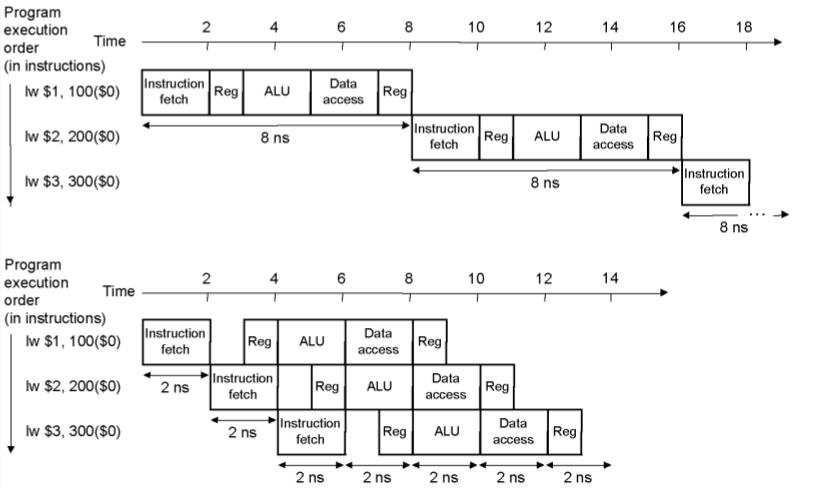
\includegraphics[scale=0.30]{images/singlevspipelined.jpg} .
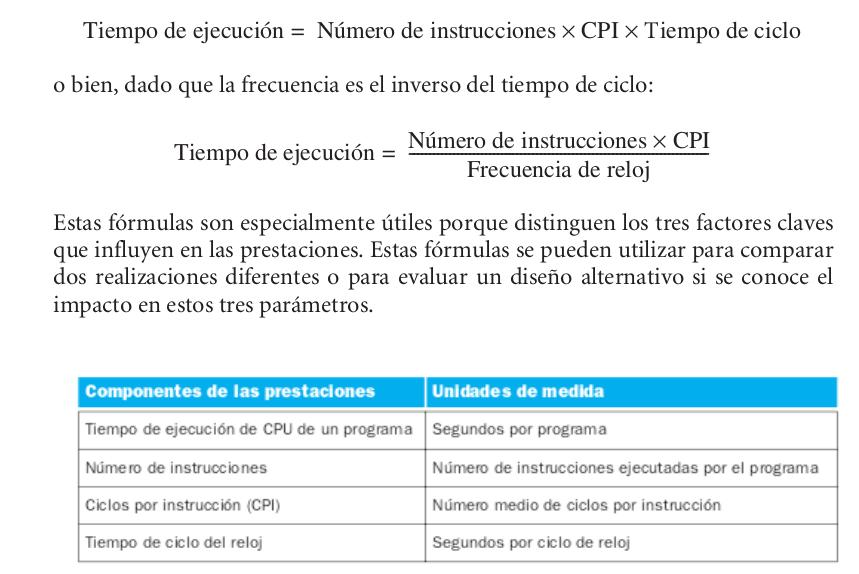
\includegraphics[scale=0.15]{images/tiempo.jpg} \\
La microarquitectura segmentada mejora la \textbf{duración del ciclo de reloj (frecuencia del reloj)}
\end{figure}
\end{frame}



\subsection{Ejemplo con una única instruccion: lw}


\begin{frame}{Ejemplo con una única instruccion: lw}{Etapas}
\begin{itemize}
\item PC es calculado en la primera etapa
\end{itemize}
\begin{figure}
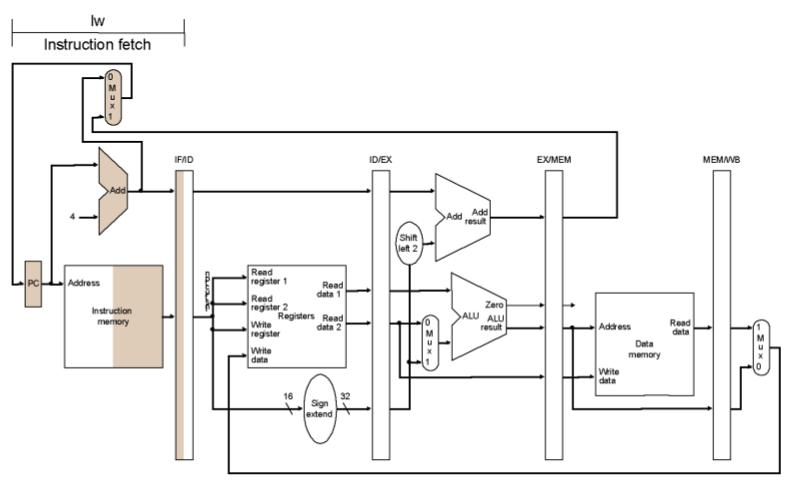
\includegraphics[scale=0.27]{images/lw1.jpg} \\
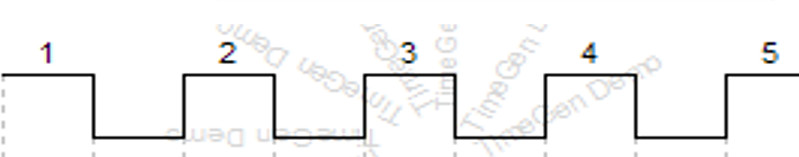
\includegraphics[scale=0.27]{images/clock2.jpg} 
\end{figure}

\end{frame}



\begin{frame}{Ejemplo con una única instruccion: lw}{Etapas}
\begin{itemize}
\item Decodificar la instrucción
\item Leer datos del archivo de registros
\end{itemize}
\begin{figure}
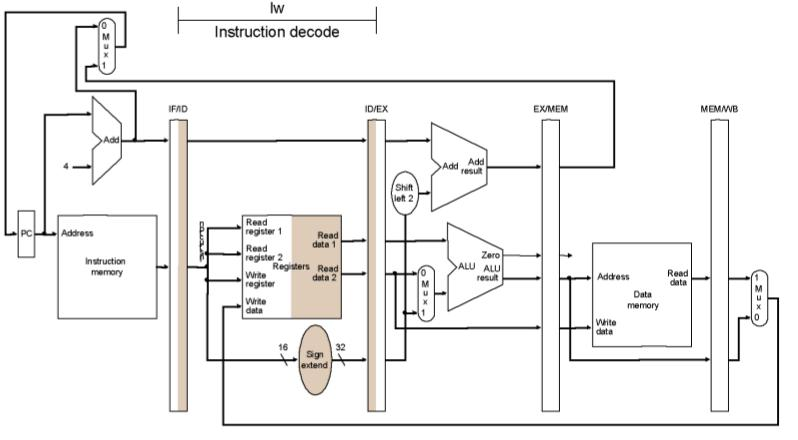
\includegraphics[scale=0.27]{images/lw2.jpg} \\
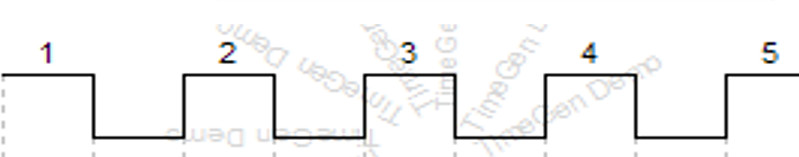
\includegraphics[scale=0.27]{images/clock2.jpg} 
\end{figure}

\end{frame}




\begin{frame}{Ejemplo con una única instruccion: lw}{Etapas}
\begin{itemize}
\item Calculo de la dirección efectiva
\end{itemize}
\begin{figure}
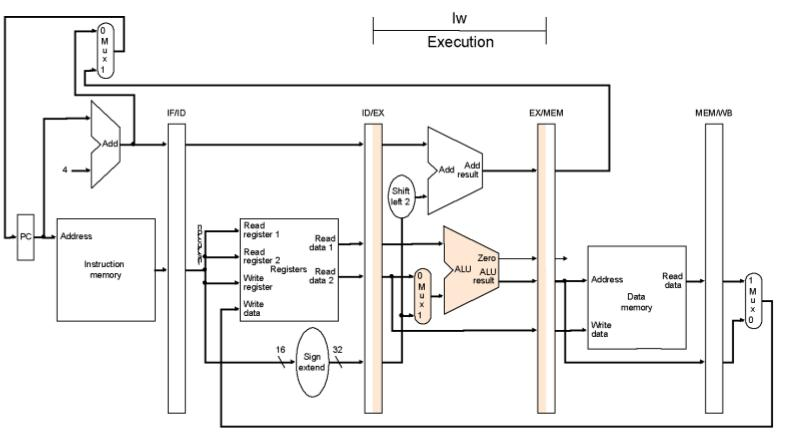
\includegraphics[scale=0.27]{images/lw3.jpg} \\
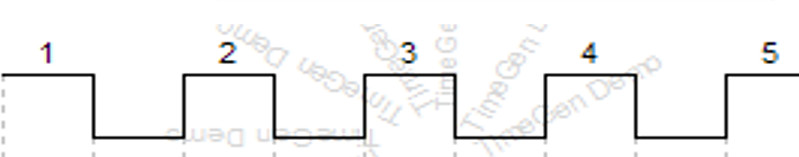
\includegraphics[scale=0.27]{images/clock2.jpg} 
\end{figure}

\end{frame}



\begin{frame}{Ejemplo con una única instruccion: lw}{Etapas}
\begin{itemize}
\item Acceso a la memoria de datos
\end{itemize}
\begin{figure}
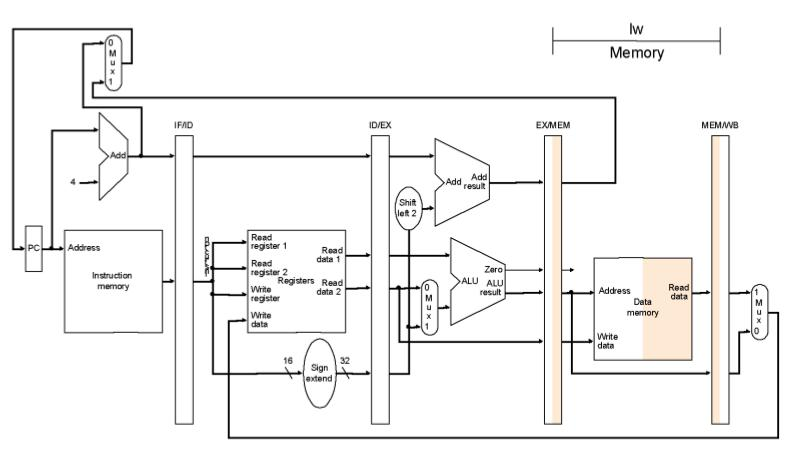
\includegraphics[scale=0.27]{images/lw4.jpg} \\
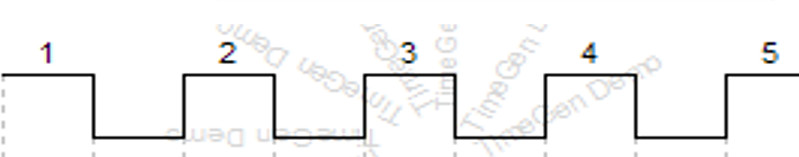
\includegraphics[scale=0.27]{images/clock2.jpg} 
\end{figure}

\end{frame}







\begin{frame}{Ejemplo con una única instruccion: lw}{Etapas}
\begin{itemize}
\item Escritura del dato en el archivo de registros
\end{itemize}
\begin{figure}
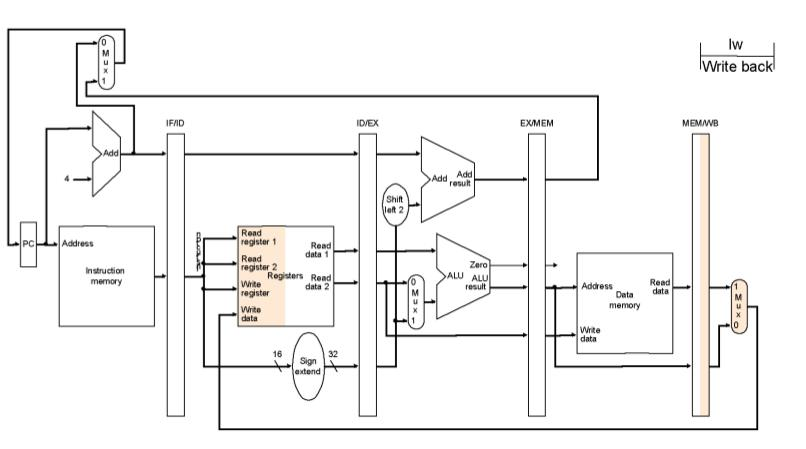
\includegraphics[scale=0.27]{images/lw5.jpg} \\
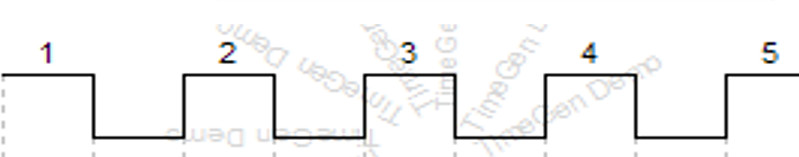
\includegraphics[scale=0.27]{images/clock2.jpg} 
\end{figure}

\end{frame}



\begin{frame}{Ejemplo con una única instruccion: lw}{Etapas}
\begin{itemize}
\item \textbf{¿Cómo pueden llegar las señales del registro destino?}
\end{itemize}
\begin{figure}
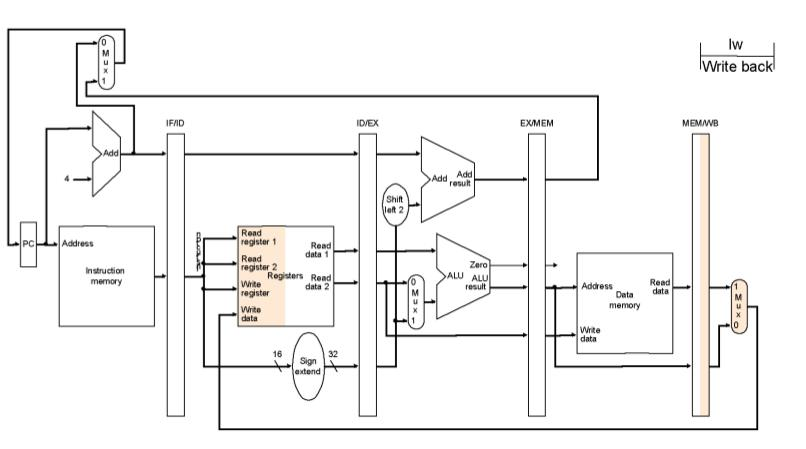
\includegraphics[scale=0.4]{images/lw5.jpg} 
\end{figure}

\end{frame}





\begin{frame}{Ejemplo con una única instruccion: lw}{Etapas}
\begin{itemize}
\item \textbf{¿Cómo pueden llegar las señales del registro destino?}
\item Utilizando registros de la microarquitectura entre las etapas
\item Las señales son copiadas entre las etapas
\end{itemize}
\begin{figure}
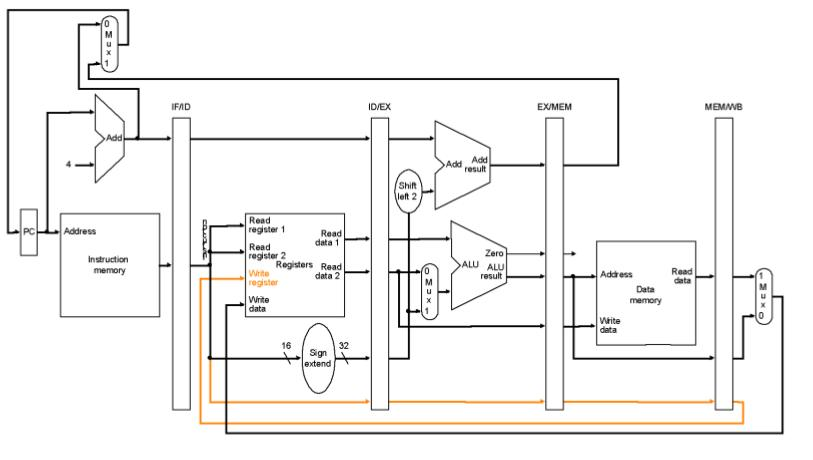
\includegraphics[scale=0.3]{images/sw.jpg} 
\end{figure}

\end{frame}



\begin{frame}
\frametitle{Implementación de la Microarquitectura}
\begin{center}\textbf{Representación visual del camino segmentado}\end{center}
\begin{itemize}
\item Orientado a los recursos utilizados
\item Diagrama simplificado
\end{itemize}
\begin{figure}
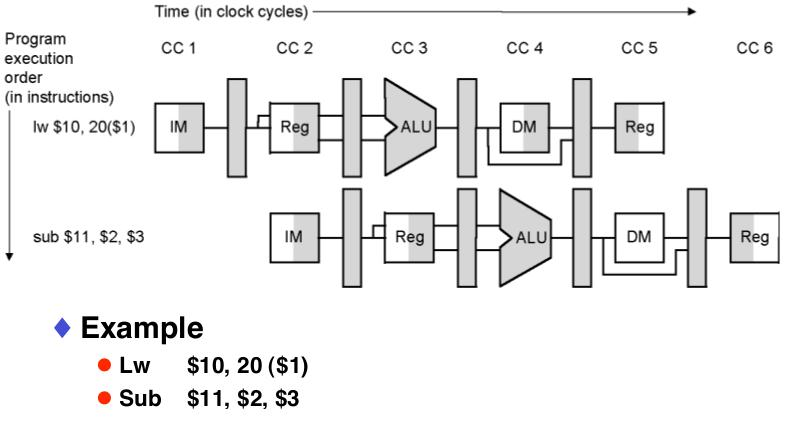
\includegraphics[scale=0.3]{images/dosinstrucciones.jpg} 
\end{figure}

\end{frame}

\subsection{Unidad de Control: generación de señales}

\begin{frame}
\frametitle{Implementación de la Microarquitectura}
\begin{center}\textbf{Unidad de control: generación de las señales}\end{center}
\begin{figure}
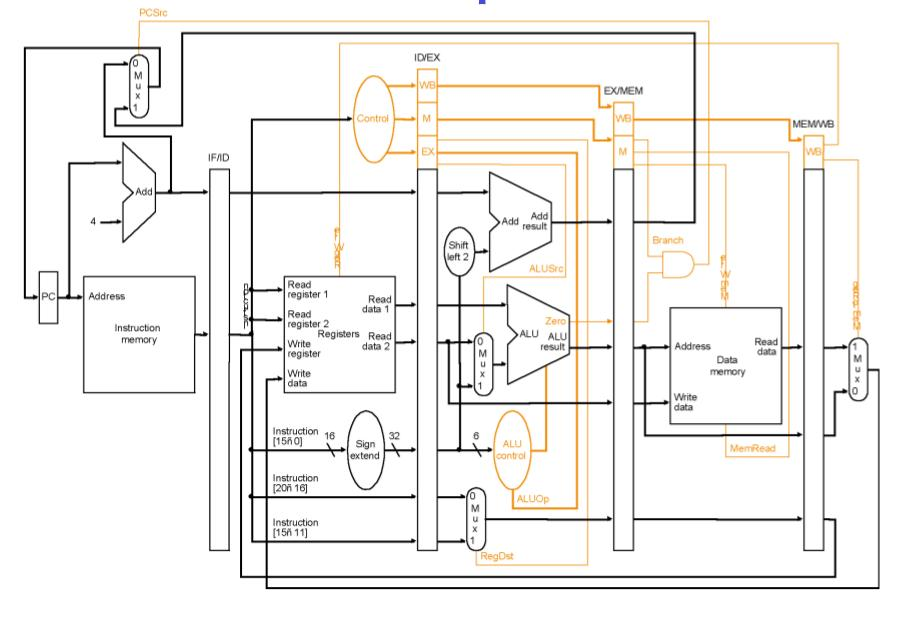
\includegraphics[scale=0.30]{images/control.jpg} 
\end{figure}

\end{frame}

















\subsection{Ejemplo de una secuencia de instrucciones}




\begin{frame}
\frametitle{Implementación de la Microarquitectura}
\begin{center}\textbf{Ejemplo de una secuencia de instrucciones}\end{center}

\begin{itemize}
\item lw \$10, 20 (\$1)
\item sub \$11, \$2, \$3
\item and \$12, \$4, \$5
\item or \$13, \$6, \$7
\item add \$14, \$8, \$9
\end{itemize}

\end{frame}








\begin{frame}{Ejemplo de una secuencia de instrucciones}{Segmentación (Pipeling)}

 \begin{columns}[onlytextwidth,T]
      \column{\dimexpr\linewidth-110mm-5mm}

\bigskip
\begin{itemize}
\item lw \$10, 20 (\$1)
\item sub \$11, \$2, \$3
\item and \$12, \$4, \$5
\item or \$13, \$6, \$7
\item add \$14, \$8, \$9
\end{itemize}

      \column{100mm}
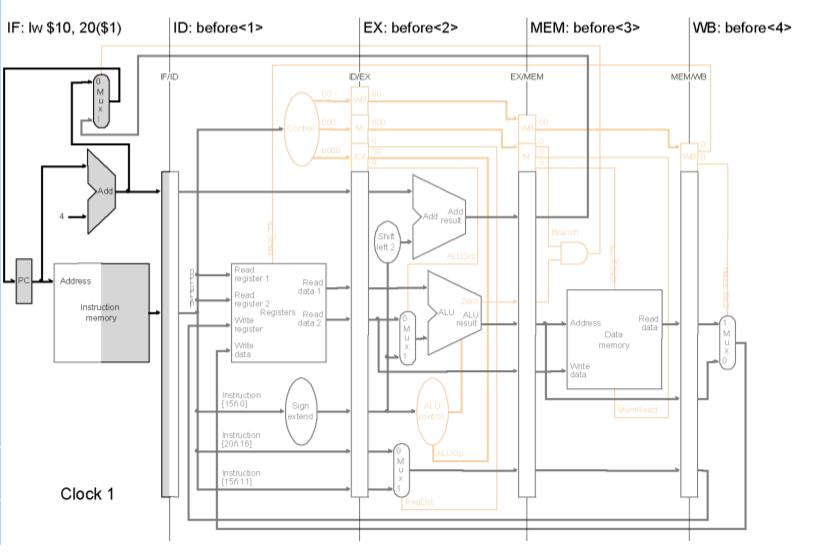
\includegraphics[scale=0.35]{images/pipeling1.jpg} 
    \end{columns}

\end{frame}


\begin{frame}{Ejemplo de una secuencia de instrucciones}{Segmentación (Pipeling)}

 \begin{columns}[onlytextwidth,T]
      \column{\dimexpr\linewidth-110mm-5mm}

\bigskip
\begin{itemize}
\item lw \$10, 20 (\$1)
\item sub \$11, \$2, \$3
\item and \$12, \$4, \$5
\item or \$13, \$6, \$7
\item add \$14, \$8, \$9
\end{itemize}

      \column{100mm}
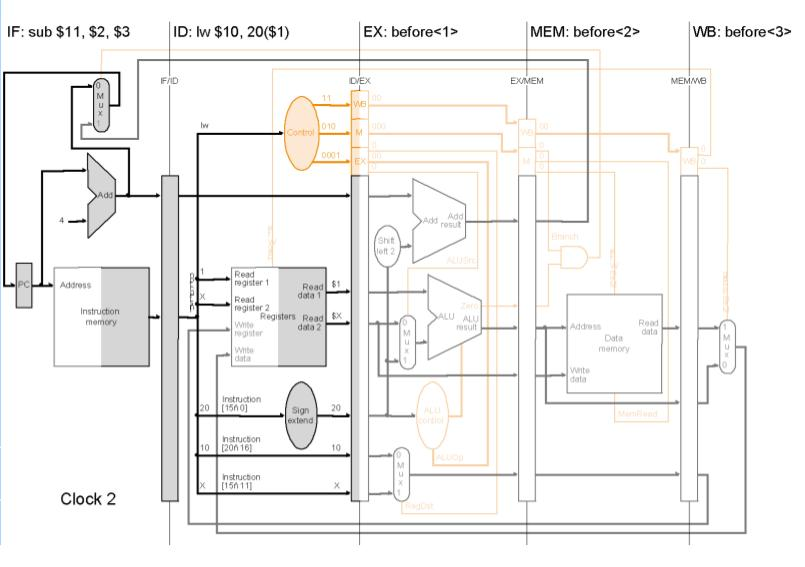
\includegraphics[scale=0.35]{images/pipeling2.jpg} 
    \end{columns}

\end{frame}


\begin{frame}{Ejemplo de una secuencia de instrucciones}{Segmentación (Pipeling)}

 \begin{columns}[onlytextwidth,T]
      \column{\dimexpr\linewidth-110mm-5mm}

\bigskip
\begin{itemize}
\item lw \$10, 20 (\$1)
\item sub \$11, \$2, \$3
\item and \$12, \$4, \$5
\item or \$13, \$6, \$7
\item add \$14, \$8, \$9
\end{itemize}

      \column{100mm}
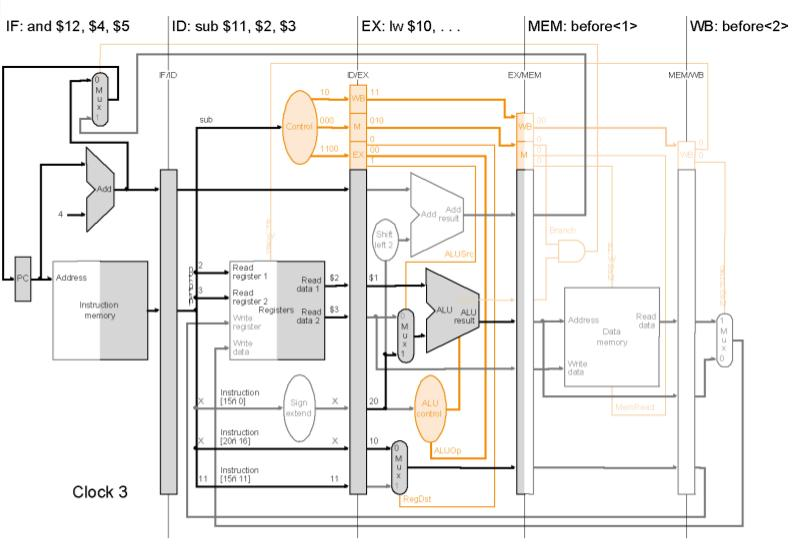
\includegraphics[scale=0.35]{images/pipeling3.jpg} 
    \end{columns}

\end{frame}

\begin{frame}{Ejemplo de una secuencia de instrucciones}{Segmentación (Pipeling)}

 \begin{columns}[onlytextwidth,T]
      \column{\dimexpr\linewidth-110mm-5mm}

\bigskip
\begin{itemize}
\item lw \$10, 20 (\$1)
\item sub \$11, \$2, \$3
\item and \$12, \$4, \$5
\item or \$13, \$6, \$7
\item add \$14, \$8, \$9
\end{itemize}

      \column{100mm}
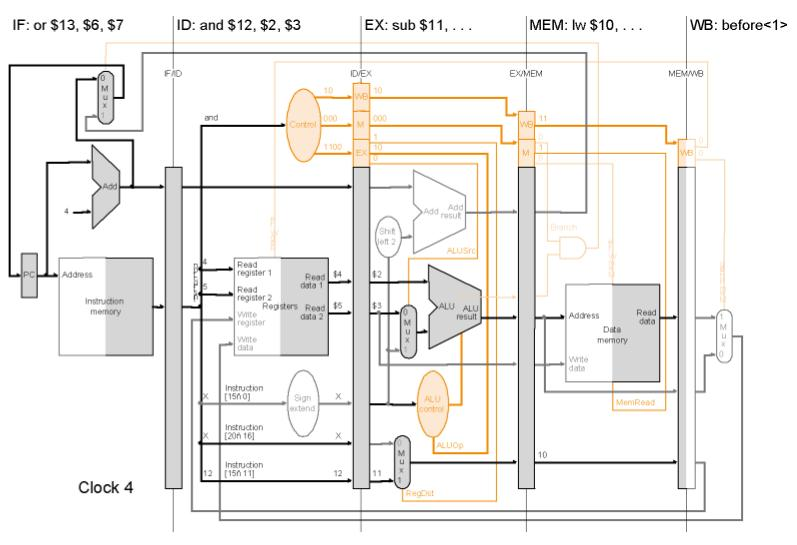
\includegraphics[scale=0.35]{images/pipeling4.jpg} 
    \end{columns}

\end{frame}

\begin{frame}{Ejemplo de una secuencia de instrucciones}{Segmentación (Pipeling)}

 \begin{columns}[onlytextwidth,T]
      \column{\dimexpr\linewidth-110mm-5mm}

\bigskip
\begin{itemize}
\item lw \$10, 20 (\$1)
\item sub \$11, \$2, \$3
\item and \$12, \$4, \$5
\item or \$13, \$6, \$7
\item add \$14, \$8, \$9
\end{itemize}

      \column{100mm}
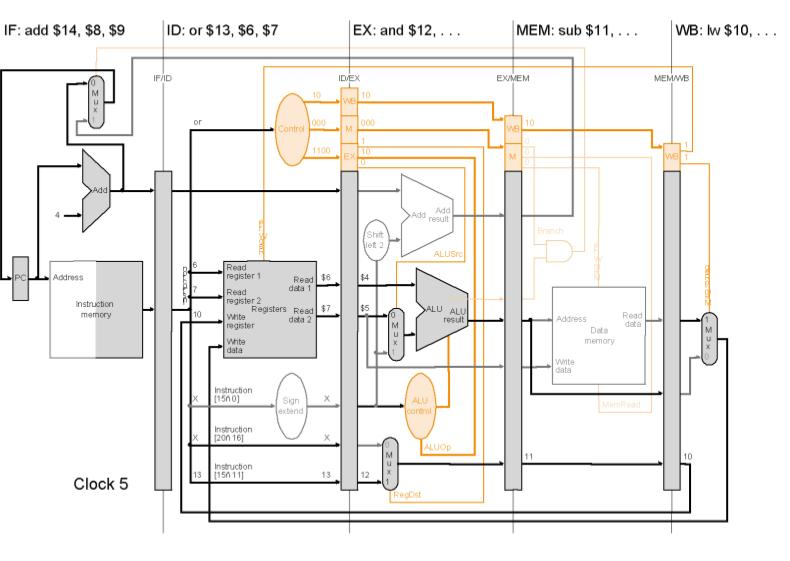
\includegraphics[scale=0.35]{images/pipeling5.jpg} 
    \end{columns}

\end{frame}

\begin{frame}{Ejemplo de una secuencia de instrucciones}{Segmentación (Pipeling)}

 \begin{columns}[onlytextwidth,T]
      \column{\dimexpr\linewidth-110mm-5mm}

\bigskip
\begin{itemize}
\item lw \$10, 20 (\$1)
\item sub \$11, \$2, \$3
\item and \$12, \$4, \$5
\item or \$13, \$6, \$7
\item add \$14, \$8, \$9
\end{itemize}

      \column{100mm}
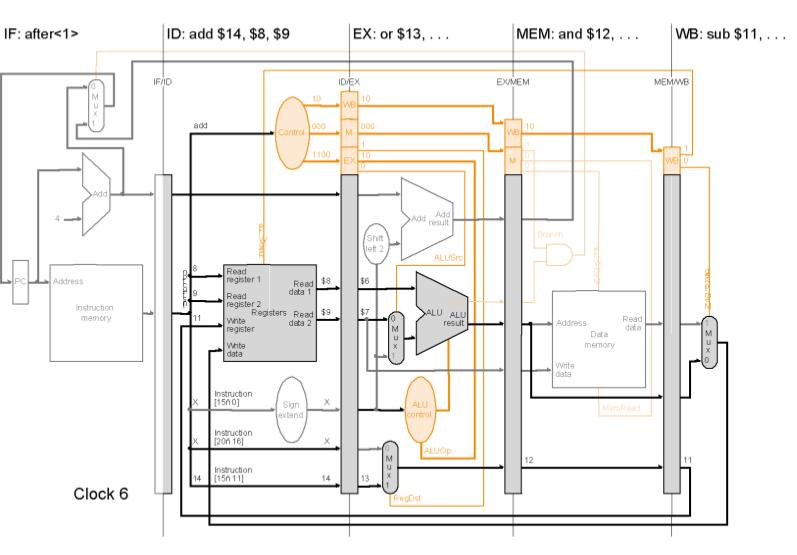
\includegraphics[scale=0.35]{images/pipeling6.jpg} 
    \end{columns}

\end{frame}

\begin{frame}{Ejemplo de una secuencia de instrucciones}{Segmentación (Pipeling)}

 \begin{columns}[onlytextwidth,T]
      \column{\dimexpr\linewidth-110mm-5mm}

\bigskip
\begin{itemize}
\item lw \$10, 20 (\$1)
\item sub \$11, \$2, \$3
\item and \$12, \$4, \$5
\item or \$13, \$6, \$7
\item add \$14, \$8, \$9
\end{itemize}

      \column{100mm}
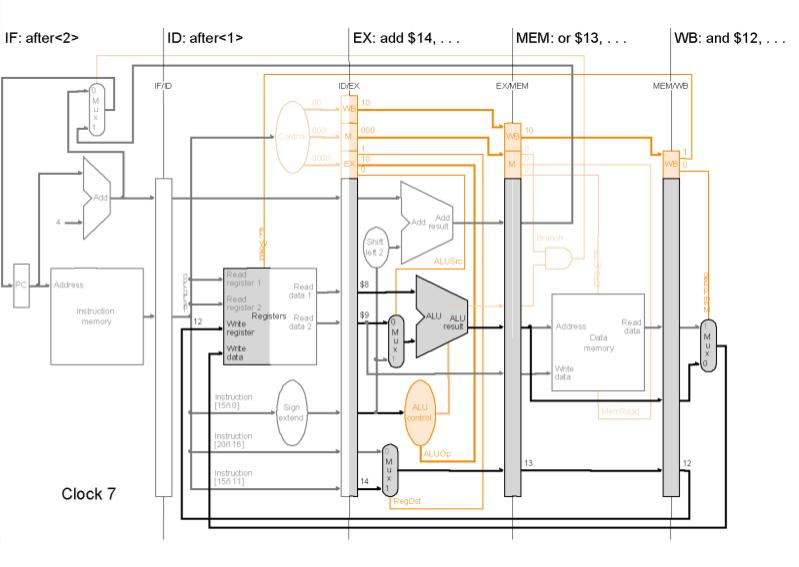
\includegraphics[scale=0.35]{images/pipeling7.jpg} 
    \end{columns}

\end{frame}

\begin{frame}{Ejemplo de una secuencia de instrucciones}{Segmentación (Pipeling)}

 \begin{columns}[onlytextwidth,T]
      \column{\dimexpr\linewidth-110mm-5mm}

\bigskip
\begin{itemize}
\item lw \$10, 20 (\$1)
\item sub \$11, \$2, \$3
\item and \$12, \$4, \$5
\item or \$13, \$6, \$7
\item add \$14, \$8, \$9
\end{itemize}

      \column{100mm}
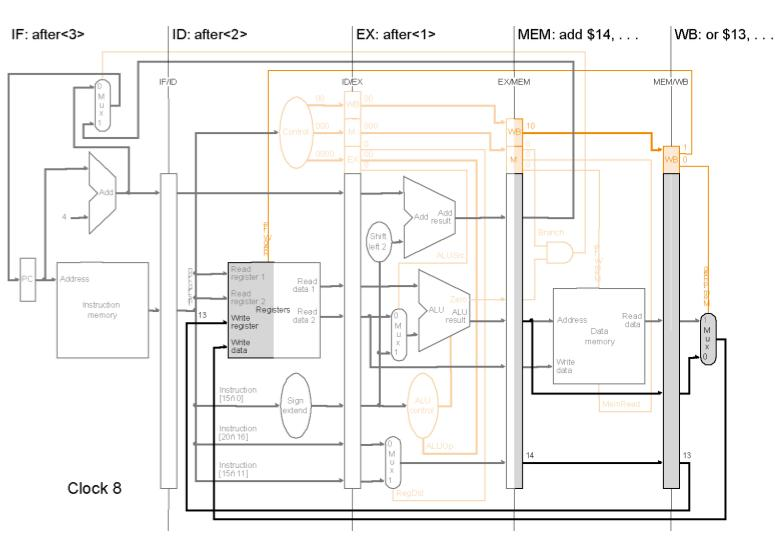
\includegraphics[scale=0.35]{images/pipeling8.jpg} 
    \end{columns}

\end{frame}

\begin{frame}{Ejemplo de una secuencia de instrucciones}{Segmentación (Pipeling)}

 \begin{columns}[onlytextwidth,T]
      \column{\dimexpr\linewidth-110mm-5mm}

\bigskip
\begin{itemize}
\item lw \$10, 20 (\$1)
\item sub \$11, \$2, \$3
\item and \$12, \$4, \$5
\item or \$13, \$6, \$7
\item add \$14, \$8, \$9
\end{itemize}

      \column{100mm}
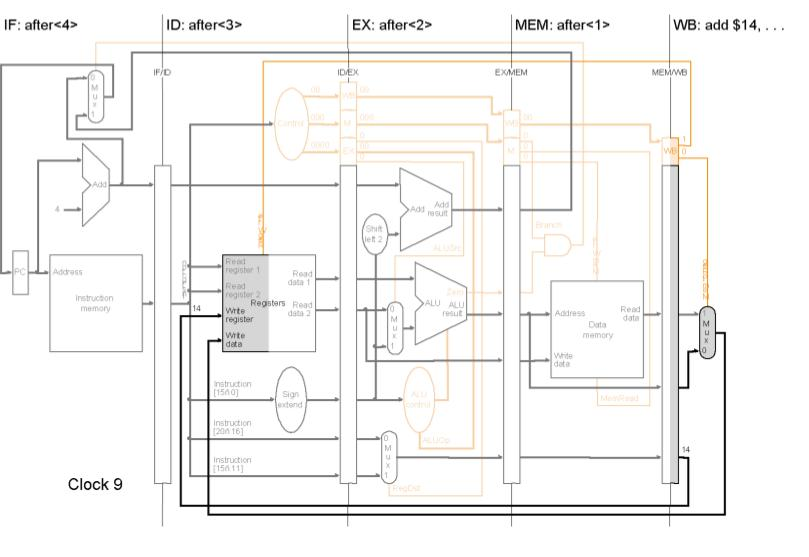
\includegraphics[scale=0.35]{images/pipeling9.jpg} 
    \end{columns}

\end{frame}













\subsection{Problemas que surgen con la segmentación (HAZARDS)}



\begin{frame}{Problemas de la segmentación (HAZARDS)}{y sus soluciones o alternativas}

\begin{itemize}
\item Estructurales: dos o más instrucciones intentando utilizar una misma unidad
\item Datos: dependencias
\end{itemize}

Formas de tratarlos
\begin{itemize}
\item Compilador
\begin{itemize}
\item Reordenar instrucciones
\item Agregar detenciones (instrucciones nop)
\end{itemize}
\item Unidad de control
\begin{itemize}
\item Detectar el problema (hazard)
\item Realizar una o más detenciones (stall), o 
\item Reenvío de señales entre etapas (Forwarding)
\end{itemize}
\end{itemize}

\end{frame}



\begin{frame}{Problemas de la segmentación (HAZARDS)}{y sus soluciones o alternativas}
\begin{center}\textbf{Ejemplo de una dependencia de datos (data hazard)}\end{center}
Secuencia de instrucciones
\begin{figure}
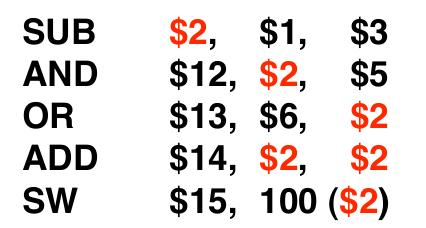
\includegraphics[scale=0.35]{images/pipeling-hazard1.jpg} 
\end{figure}

\end{frame}


\begin{frame}{Problemas de la segmentación (HAZARDS)}{y sus soluciones o alternativas}
\begin{center}\textbf{Ejemplo de una dependencia de datos (data hazard)}\end{center}
Visión del problema en el camino de datos
\begin{figure}
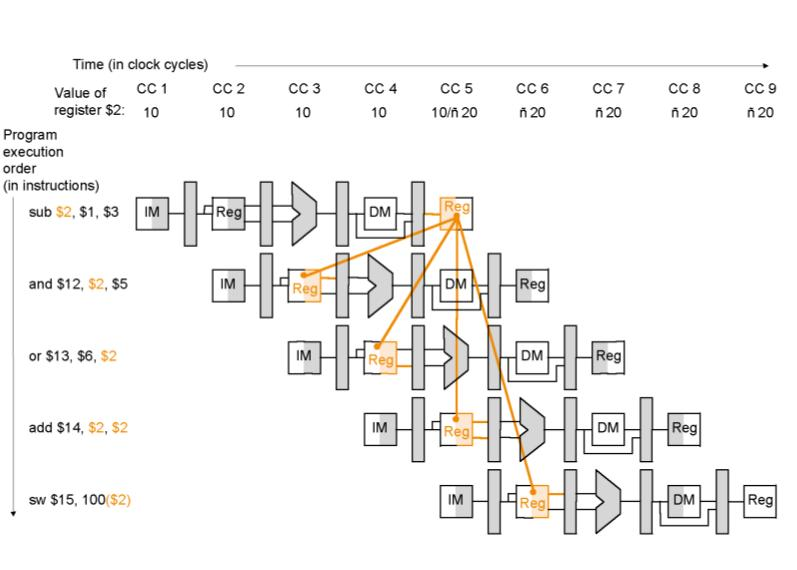
\includegraphics[scale=0.35]{images/pipeling-hazard2.jpg} 
\end{figure}

\end{frame}



\begin{frame}{Problemas de la segmentación (HAZARDS)}{y sus soluciones o alternativas}
\begin{center}\textbf{Ejemplo de una dependencia de datos (data hazard)}\end{center}
Solución 1: Resuelta por el compilador puede demorar algunas instrucciones
\begin{figure}
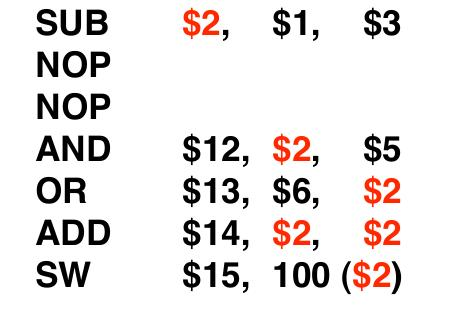
\includegraphics[scale=0.35]{images/pipeling-hazard3.jpg} 
\end{figure}

\end{frame}


\begin{frame}{Problemas de la segmentación (HAZARDS)}{y sus soluciones o alternativas}
\begin{center}\textbf{Ejemplo de una dependencia de datos (data hazard)}\end{center}
Solución 1: Unidad de control mas compleja (forwarding)
\begin{figure}
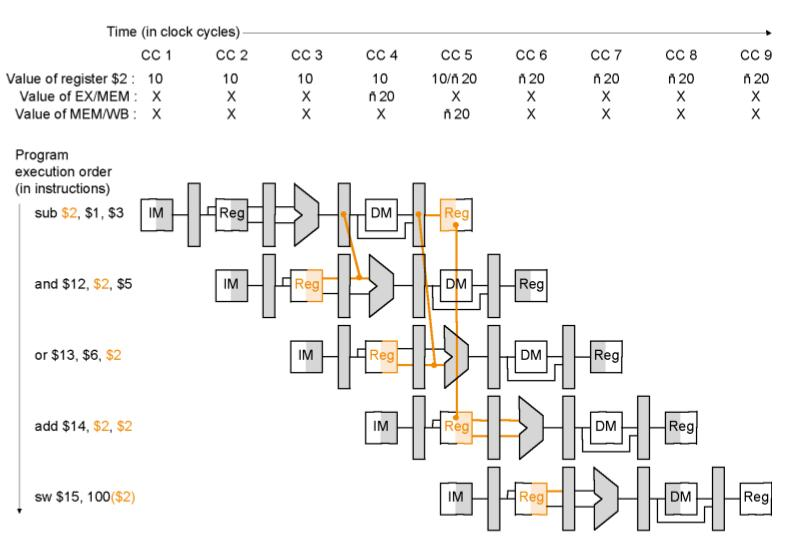
\includegraphics[scale=0.35]{images/pipeling-hazard4.jpg} 
\end{figure}

\end{frame}


\begin{frame}{Hazards: Cuando no puede evitarse la detencción}
\begin{itemize}
\item Delay slot: Se necesita una solución arquitectural (en MIPS lo soluciona el compilador)
\item Dependencias inevitables (el dato no está disponible en ninguna etapa)
\end{itemize}

\end{frame}


\begin{frame}
 \frametitle{Consejos y preguntas}
\begin{center}
\begin{itemize}
\item  ¿Preguntas?
\end{itemize}
\end{center}
\end{frame}


\begin{frame}
 \frametitle{Bibliografía}
Libros
\begin{itemize}
\item David. Patterson John L. Hennessy (1995), ORGANIZACIÓN Y DISEÑO DE COMPUTADORES La interfaz hardware/software, McGraw-Hill (8 copias en biblioteca).
\end{itemize}
\end{frame}

\end{footnotesize}

\end{document}
